\chapter{Experimental Design} \label{ExpDesign}
In this Chapter, the datasets are selected, general design ideas are explained and established, global hyper-parameters are defined and at last the experiments and their goals are described.

\section{Tools}
The following Sections provide insight on what tools, such as software and hardware, is used to conduct the experiments.

\subsection{Hardware}
All experiments are conducted on a HP Probook equipped with a Intel Core i7 with 2.8GHz and 32GB of RAM installed. No additional graphics card was used.

\subsection{Software}
All necessary code is written in R (Version 4.1.0). To design the neural networks, the library Keras (Version 2.4.0) together with the Tensorflow (Version 2.5.0) backend is used.


\section{Datasets}
Following, it is motivated how and why the proposed data sets are used.

\subsection{Problems of Existing Benchmarks} \label{Problems of Existing Benchmarks}
In order to find out, which neural network architecture is better suited for anomaly detection, first, suitable datasets have to be evaluated. Most of the papers on anomaly detection test on one of the popular benchmark datasets such as the ones created by Numenta, Yahoo,  which are used by Braei and Wagner \parencite{Braei2020}, NASA, or Pei's Lab. These benchmark datasets are, however, declared as flawed by Wu and Keogh \parencite*{Wu2020}. Wu and Keogh \parencite*{Wu2020} state that the benchmark datasets suffer from at least one of the following flaws:

\begin{enumerate}
	\item \textbf{Triviality:} Surprisingly, a sizable proportion of the problems in the benchmark datasets are trivial to solve. Triviality is hereby defined as follows: An anomaly can be found with just one line of code.
	\item \textbf{Unrealistic Density:} This flaw refers to too many anomalies in the dataset or at least in a certain region, whereas in a real-world dataset the anomalous data points make up a portion of just above 0 percent.   
	\item \textbf{Mislabelled Ground Truth:} The data in all of the benchmark datasets appears to be mislabelled, with both false positives and false negatives. This is significant for a number of reasons. The majority of anomaly detectors work by computing statistics for each subsequence of some length. They may, however, place their computed label at the beginning, end, or middle of the subsequence. If caution is not exercised, an algorithm may be penalized for reporting a positive just to the left or right of a labelled region.
	\item \textbf{Run-to-failure Bias:} Because many real-world systems are run-to-failure, there is often no data to the right of the last anomaly. Therefore, a naïve algorithm that labels the last point as an anomaly has a very good chance of being correct.
\end{enumerate}

In their work, Wu and Keogh \parencite*{Wu2020}, introduced the UCR Time Series Anomaly Datasets as new benchmark, that avoids the problems listed above. However, at the start of this research project the datasets were not publicly available. Because the search for a dataset, that does not suffer from the above mentioned flaws, would be too time-consuming, the decision was taken to partly engineer own datasets.
\newline
\subsection{Anomalies}
The neural networks should be used to detect various types of anomalies, in order to test their ability to recognize them. Foorthuis \parencite*{Foorthuis2021} compiled, in an extensive literature review, a study on the different types of anomalies. The anomalies were divided into different categories, of which foremost the quantitative multivariate aggregate anomalies are relevant for this research project, especially a) to f) (see figure \ref{fig:Anomaly_types}). These types of anomalies typically occur in time series data, that is composed by sensor data. Examples of such data could be temperature measurements or Electrocardiograms \parencite{Malhotra2015}.

\begin{figure}[h]
	\centering
	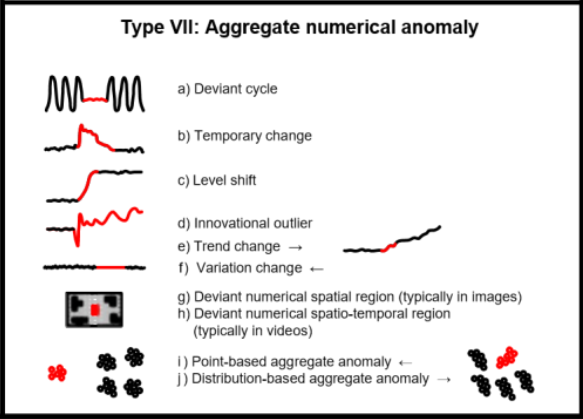
\includegraphics[scale=0.6]{Figures/series_anomaly}
	\decoRule
	\caption[Quantitative Anomalies]{Quantitative Anomalies \parencite{Foorthuis2021}}
	\label{fig:Anomaly_types}
	%https://arxiv.org/ftp/arxiv/papers/2007/2007.15634.pdf
\end{figure}

\subsection{Dataset Selection}
In the following subsections, it is proposed how and why the datasets are selected for the different experiments.

\subsubsection{1. Dataset}
The dataset, which should be used for the first experiment will be of synthetic nature. It consists of various cyclic patterns. In a second step, the dataset is enriched with anomalies. This way, two datasets are produced. The dataset without anomalies is used for an unsupervised learning approach, whereas the dataset with labelled anomalies is used for a supervised approach. Further information, on how the dataset is created, on the temporal behaviour and what the anomalies look like can be found in Section \ref{dataset1} 

\subsubsection{2. Dataset}
The second dataset, which is used for anomaly detection, consists of real sensor data. To make sure, that the requirements, mentioned in section \ref{Problems of Existing Benchmarks} are met as closely as possible, the anomalies are engineered and embedded manually into the dataset. 

\subsubsection{3. Dataset}
As third dataset, one of the existing benchmark datasets should be used. Despite their obvious flaws, it is still considered useful to validate the previously achieved results on an official benchmark. Further, this gives insights into the overall usefulness of the proposed neural network architectures as the achieved result can be compared to previous experiments.

\subsection{Split of Datasets}
The conventional train, validate, and test dataset technique is used with all datasets.
This method is widely used in machine learning. The training set is hereby used to fit the model. The validation set is used to provide an unbiased evaluation of the model fit on the training dataset while tuning the hyper-parameters. The test set is then used to offer an objective assessment of the final model \parencite{Brownlee2017}. For the supervised approach, the training dataset is enriched with anomalies, whereas for the unsupervised approach a "clean" dataset is used. The final evaluation is done on a test dataset, which is the same for the supervised and unsupervised approaches.


\section{Setup of Experiments} \label{SetupOfExperiments}
The following section explains how the different experiments are conducted in detail. When designing the experiments, the focus is put on comparability rather than optimally tuned neural networks.  Further, it is shown how the datasets and anomalies were engineered.

The following subsections give information on the chosen setups of the experiments that apply to \textbf{all} experiments. Further, global hyper-parameters are defined. Global hyper-parameters are defined manually and are the same for all experiments. Hyper-parameters, which do not fall in this category such as number of neurons in a layer, are specified in Chapter \ref{Experiments} in the section belonging to the respective experiment.

\subsection{Supervised Learning}
The supervised learning approach refers to training the neural network on a labelled dataset. The dataset used for training already has the anomalies embedded. The task of finding the anomalies can also be described as a classification task, where the neural networks classify a sequence as normal or anomalous. In such a case binary crossentropy and a sigmoid activation function are used as loss function and last layer activation fuction \parencite{Brownlee2019}. The aforementioned combination means that in the last layer a logistic regression (see Appendix \ref{logitRegression}) is done, where a threshold is determined to classify the sequences into normal and anomalous.

Supervised classification tasks are used and function well when sufficient samples of all classes are available. In anomaly detection, this is generally not the case, as the anomalous is per definition underrepresented. In the literature (e.g. \parencite{Wen2019}), however, the supervised approach is still successfully used. There are two explanations for this: First, as explained in Section \ref{Problems of Existing Benchmarks}, the density of anomalies is unrealistic and second, the anomalies are of the same kind and always look very similar, so a neural network is able to learn the pattern of the anomaly. In the experiments it is investigated, how the neural networks react when presented with anomalies that are similar to the ones in the training data, but also to previously unseen anomalies of the same kind (e.g. level shift). It is expected that any neural network will fail when there are not enough similar anomalies in the training data.

\subsection{Unsupervised Learning}
The unsupervised learning approach refers to the training of a neural network on a dataset that is free of anomalies. The neural network merely learns the cyclic pattern of the data. When learning the pattern, the loss function applied is Mean Absolute Error (MAE), so the learning task is a regression, which itself is supervised \parencite{Brownlee2019}. The actual anomaly detection hereby is done in a second step. As proposed in Section \ref{CNN on univariate series} by Munir et. al \parencite*{Munir2019}, the anomaly detector module, which is also used in this work, calculates the Euclidean distance between predicted and actual value, where a large value corresponds to an anomaly.

A unsupervised approach is the more reliable choice when trying to detect anomalies, because the model does not need to know what anomalies might look like. However, setting up this approach is more time consuming, especially when dealing with multivariate time series, as for every variable, a separate detector module and corresponding threshold needs to be set up. It is yet expected, that both neural network architectures, CNN and RNN, will outperform their supervised counterparts. 

\subsection{Neural Networks}
The following Sections describe principles that will be used in the design of the neural networks. The described principles and their corresponding hyperparamters are used in all experiments. Parameters that are specific to the experiment are specified in the corresponding section in the Chapter \ref{Experiments}. 

\subsubsection{Normalization}
Before the data is fed into the neural network it is normalized. Normalization ensures that the magnitude of the values that a feature assumes are more or less the same. Therefore, the mean of each time series is subtracted of each time series and divided by the standard deviation \parencite{Stöttner2019}. As normalization parameters, the mean and standard deviation calculated on the training set was used for all, test, validation and training dataset.  
%https://towardsdatascience.com/why-data-should-be-normalized-before-training-a-neural-network-c626b7f66c7d

\subsubsection{Activation Function}
When designing the neural networks, as activation function generally "ReLu" (Rectified Linear Unit) is used. The function is non-linear and basically just returns the input if it is bigger than 0 and otherwise 0. This function is widely used, because of its simplicity and generally yields good results with little computation expenses \parencite{Brownlee2019.2}.  

\subsubsection{Optimizer}
As optimizer, the often-used default choice in machine learning, ADAM (Adaptive Moment Estimation), with the proposed default values, is applied \parencite{Katanforoosh2019}. ADAM updates the learning rate when training, making it faster than other optimizers such a Gradient Descent. On the downside, however, ADAM uses a lot memory for a given batch size and is found to generalize poorly in late stages of training.
%https://www.deeplearning.ai/ai-notes/optimization/ 

\subsubsection{Batch Computing}
%https://medium.com/analytics-vidhya/when-and-why-are-batches-used-in-machine-learning-acda4eb00763
Typically, in machine learning, training examples are not used one after another or all at once, because updating the optimizer function after every example or only after the whole dataset is inefficient as it uses a lot of memory. To speed up the process, training data is fed to the machine learning model in batches. A batch is a collection of training examples. The size of these batches, however, also has an impact on the learning ability of the machine learning model. When using an ADAM optimizer, too large batches can have a negative impact on performance of the model \parencite{Krishnan2019}.\\
When detecting anomalies, the batch size parameter is only used when training. As in a real-world scenario every new measurement is analysed immediately since it mostly is crucial to detect the anomaly as early as possible. Analysing every datapoint, however, leads to a increase in computation time which explains the long inference times in the experiments.
% no batch computing on test sets, because you would not wait for a batch to be complete and just calculate the anomaly score straigth away

\subsection{Experiments}
In the following, it is suggested how the experiments on the 3 different datasets are conducted.

\subsubsection{1. Experiment}
In a first experiment the learning abilities of RNN and CNN are compared. It is investigated how useful the architectures are in a supervised and in an unsupervised setup. This experiment gives general insight on which setups and approaches work under which conditions. As the anomalies embedded are similar in the training and test set, the supervised approaches should yield good results, whereas the unsupervised approaches, given the simplicity of the dataset, are not expected to miss any anomalies.

\subsubsection{2. Experiment}
The second experiment is conducted on a more challenging dataset. Also, the embedded anomalies are of a more challenging nature. All approaches that have been found successful in Experiment 1, are investigated further on the new dataset. Since the dataset consists of more, partially dependent, variables, and more challenging cyclic patterns the architectures used in Experiment 1 may be extended for example by adding additional layers. 

\subsubsection{3. Experiment}
In the third experiment, a dataset that has already been used in the field of anomaly detection should be used. The neural network architecture types, CNN and RNN, are applied to the chosen dataset. First, this shows which approach is better suited and second, the achieved results can be compared to already existent results to verify the overall performance of the chosen anomaly detection methods.

\subsection{Results}
As results three metrics are reported. First and most important, is the F1-Score which gives insight on the models ability to recognize anomalies. The F1-Score is preferred over the AUC, because it is more significant on imbalanced datasets \parencite{Forman2010}. The F1-Score provides a better estimate of how many anomalies are correctly identified. As it is assumed that a model properly classifies a significant number of true negatives. Therefore, AUC-Score of the models would be very high and similar and thus harder to compare. The other two metrics reported of each model are the training and inference time.



 